\documentclass{article}

\usepackage[utf8]{inputenc}
\usepackage[T1]{fontenc}
\usepackage[hmargin=2.5cm,vmargin=3cm,bindingoffset=0.5cm]{geometry}

\usepackage{amsmath,amssymb}

\usepackage{graphicx}
\graphicspath{{figures/}}

\usepackage{float}
\usepackage{caption}
\usepackage{subcaption}

\usepackage{tikz}
\usetikzlibrary{arrows.meta, positioning, shapes.symbols}

\usepackage{xcolor,listings}
\definecolor{codegray}{RGB}{245,245,245}
\lstset{
  basicstyle=\ttfamily\small,
  backgroundcolor=\color{codegray},
  frame=single,
  numbers=left,
  numberstyle=\tiny,
  breaklines=true,
  captionpos=b,
  keywordstyle=\color{blue}\bfseries,
  commentstyle=\itshape\color{gray},
  stringstyle=\color{red!60!black},
  language=Python,
  literate=
    {→}{{$\rightarrow$}}2
    {≈}{{$\approx$}}2
    {≤}{{$\leq$}}2
    {≥}{{$\geq$}}2
    {–}{{--}}1
    {—}{{---}}1
}

\usepackage{booktabs}
\usepackage{longtable}
\usepackage{hyperref}
\hypersetup{
  colorlinks=true,
  linkcolor=blue!70!black,
  urlcolor=blue!70!black,
  citecolor=blue!70!black
}

\renewcommand{\lstlistingname}{Auflistung}

\begin{document}

\pagenumbering{alph}
\begin{titlepage}
  \begin{center}
    
\includegraphics[width=\textwidth]{THD-Logo.pdf}
    \vspace{1cm}
    \rule{\textwidth}{1mm}\\[0.3cm]
    \textsc{\scshape \huge Bachelor \,--\, Cyber Security}\\
    \rule{\textwidth}{1mm}\\[1.8cm]

    {\Large \bfseries Kryptologie 2}\\[1cm]
    {\Huge \bfseries Projektdokumentation}\\[0.5cm]
    {\Large \bfseries Cryptochallenge: CurveBall (CVE-2020-0601)}\\[2cm]

    \begin{minipage}[t]{0.45\textwidth}
      \begin{flushleft}
        \normalsize \emph{Autoren}\\
        Manuel Friedl – 1236626\\
        Christof Renner – 22301943
      \end{flushleft}
    \end{minipage}
    \hfill
    \begin{minipage}[t]{0.45\textwidth}
      \begin{flushright}
        \normalsize \emph{Betreuer}\\
        Prof.\,Dr.\,Martin Schramm
      \end{flushright}
    \end{minipage}\\[2cm]

    {\large Deggendorf, \today}
  \end{center}
\end{titlepage}

\newpage
\pagenumbering{Roman}
\tableofcontents
\newpage
\pagenumbering{arabic}

\section{Einleitung und Projektkontext}
\subsection{Motivation}
Die Schwachstelle \textbf{CurveBall} (CVE-2020-0601) in der Windows-CryptoAPI
ermöglicht es, X.509-Zertifikate mit manipulierten Elliptic-Curve-Parametern zu
signieren, sodass betroffene Windows-Versionen die Signaturen fälschlich als
gültig akzeptieren.\footnote{Microsoft Security Advisory ADV200002, 14.\,01.\,2020}
Im Modul \emph{Kryptologie 2} fehlte bislang ein modernes
Hands-On-Szenario, um diesen Fehler praktisch zu demonstrieren.

\subsection{Projektziele}
\begin{enumerate}
  \item \textbf{Didaktik}: Vollständiger Angriffszyklus von Discovery bis Exploit.
  \item \textbf{Sicherheit}: Deployment selbst muss trotz absichtlich verletzter Krypto sicher sein.
  \item \textbf{Portabilität}: Schnelle, plattformunabhängige Nutzung via Docker/Podman.
\end{enumerate}

\subsection{Bedrohungsmodell}
\begin{figure}[H]
  \centering
  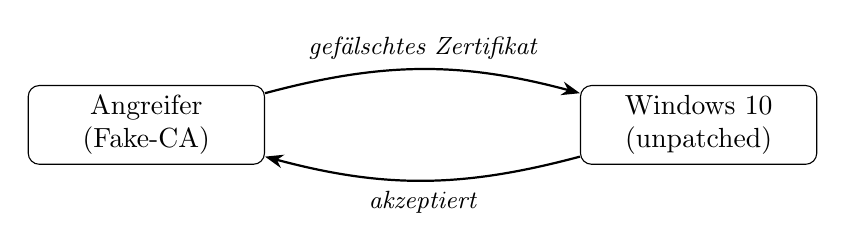
\begin{tikzpicture}[
      entity/.style={draw, rounded corners, align=center, minimum width=3cm, minimum height=1cm},
      arrow/.style={-Stealth, thick},
      label/.style={font=\small\itshape}
    ]
    \node[entity] (attacker) {Angreifer\\(Fake-CA)};
    \node[entity, right=4cm of attacker] (victim) {Windows 10\\(unpatched)};
    \path[arrow] (attacker) edge[bend left=15] node[label, above]{gefälschtes Zertifikat} (victim);
    \path[arrow] (victim) edge[bend left=15] node[label, below]{akzeptiert} (attacker);
  \end{tikzpicture}
  \caption{Simplifiziertes Threat-Model: fehlende Parameter-Validierung}
  \label{fig:threatmodel}
\end{figure}

\section{Herangehensweise}
\subsection{Zielsetzung}
\begin{itemize}
  \item Demonstration des Angriffs in einer kontrollierten Umgebung.
  \item Vermittlung von DevSecOps-Best-Practices (Linting, CI, Scans).
  \item Bereitstellung als \emph{„One-Click“}-Container, ohne lokale OpenSSL-Konfiguration.
\end{itemize}

\subsection{Methodik}
Wir arbeiteten in zwei Sprints à zwei Wochen.  
Abbildung~\ref{fig:process} zeigt den iterativen Ablauf.

\begin{figure}[H]
  \centering
  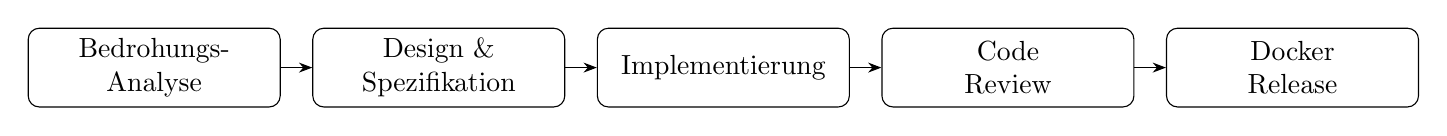
\begin{tikzpicture}[
      box/.style={draw, rounded corners, align=center, minimum width=3.2cm, minimum height=1cm},
      >=Stealth
    ]
    \node[box] (analyse) {Bedrohungs-\\Analyse};
    \node[box, right=0.4cm of analyse] (design) {Design \&\\Spezifikation};
    \node[box, right=0.4cm of design] (impl)  {Implementierung};
    \node[box, right=0.4cm of impl] (review) {Code\\Review};
    \node[box, right=0.4cm of review] (deploy) {Docker\\Release};

    \draw[->] (analyse) -- (design);
    \draw[->] (design) -- (impl);
    \draw[->] (impl) -- (review);
    \draw[->] (review) -- (deploy);
  \end{tikzpicture}
  \caption{Iterativer Projektablauf}\label{fig:process}
\end{figure}

\section{Arbeitsaufteilung}

\noindent Die Arbeitsaufteilung erfolgte pragmatisch basierend auf den individuellen Stärken der Teammitglieder, wobei gleichzeitig Wert auf Wissenstransfer und gemeinsames Lernen gelegt wurde.

\begin{longtable}{|p{3cm}|p{5cm}|p{6cm}|}
    \hline
    \textbf{Teammitglied} & \textbf{Hauptaufgaben} & \textbf{Spezifische Aufgaben} \\
    \hline
    \endhead

    Manuel Friedl & Kryptographie \& Frontend & 
    \begin{itemize}
      \item Analyse der CVE-2020-0601 Schwachstelle
      \item Entwicklung der Python-Skripte \texttt{gen\_key.py} und \texttt{simulate\_vuln\_check.py}
      \item Entwicklung des Web-Interface und Zertifikats-Visualizers
      \item Erstellung verständlicher Challenge-Beschreibungen
      \item Implementierung der Angriffslogik in Python
      \item Frontend-Design mit HTML/CSS
      \item Dokumentation der kryptographischen Konzepte
    \end{itemize} \\
    \hline

    Christof Renner & DevOps \& Infrastruktur & 
    \begin{itemize}
      \item Docker-Containerisierung mit Multi-Stage-Builds
      \item CI/CD-Pipeline mit GitHub Actions
      \item Security-Scanning und Linting-Integration
      \item GitHub Container Registry Konfiguration
      \item Dokumentation der technischen Details
      \item Container-Deployment-Architektur
      \item Implementierung der Sicherheitsmaßnahmen
      \item Frontend-Optimierungen
    \end{itemize} \\
    \hline
    \end{longtable}

\noindent Dabei wurde durch regelmäßige Abstimmungen und gemeinsame Review-Sessions sichergestellt, dass alle Komponenten nahtlos zusammenarbeiten. Die technische Dokumentation wurde gleichmäßig zwischen beiden Teammitgliedern aufgeteilt, wobei jeder etwa 50\% der Dokumentationsarbeit übernahm.

\newpage

\section{Containerisierung}
\subsection{Dockerfile}

Das Projekt nutzt ein \emph{Multi-Stage-Build}-Konzept, um die Abhängigkeiten in einem schlanken Container zu installieren und gleichzeitig die Größe des finalen Images zu minimieren. \\
Dabei wird beim starten des Containers ein einfacher HTTP-Server gestartet, der die Challenge-Dateien bereitstellt.
Die Abhängigkeiten werden in einem separaten Build-Stage installiert, um die Sicherheit und Portabilität zu erhöhen. \\
Die Abhängigkeiten sind in der Datei \texttt{requirements.txt} definiert, die die benötigten Python-Pakete enthält.

\vspace{1cm}

\begin{lstlisting}[language=bash,caption={Auszug aus dem finalen Dockerfile}]
FROM python:3.12-slim AS build
RUN apt-get update && apt-get install -y --no-install-recommends \
    libssl-dev build-essential && rm -rf /var/lib/apt/lists/*
COPY requirements.txt .
RUN pip install --prefix=/install -r requirements.txt

FROM python:3.12-slim
COPY --from=build /install /usr/local
COPY curveball-ctf /app
WORKDIR /app
USER 1001:1001
ENTRYPOINT ["python", "-m", "http.server", "8080"]
\end{lstlisting}

\subsection{Architektur}
\begin{figure}[H]
  \centering
  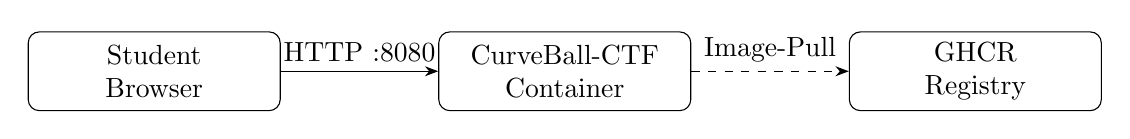
\begin{tikzpicture}[
      service/.style={draw, rounded corners, minimum width=3.2cm, minimum height=1cm, align=center},
      node distance=2cm
    ]
    \node[service] (browser) {Student\\Browser};
    \node[service, right=of browser] (ctf) {CurveBall-CTF\\Container};
    \node[service, right=of ctf] (registry) {GHCR\\Registry};

    \draw[-Stealth] (browser) -- node[midway, above]{HTTP :8080} (ctf);
    \draw[-Stealth, dashed] (ctf) -- node[midway, above]{Image-Pull} (registry);
  \end{tikzpicture}
  \caption{Container-Deployment in der Lehrumgebung}\label{fig:container}
\end{figure}

\newpage

\section{CI/CD-Pipeline}

\subsection{Docker Build-Pipeline}
\noindent
Die automatisierte Erstellung und Veröffentlichung der Docker-Images erfolgt über eine dedizierte GitHub Actions Workflow-Datei. Diese Pipeline stellt sicher, dass bei jeder Aktualisierung des Codes oder auf manuelle Anforderung ein neues, konsistentes Container-Image erstellt und in die Docker Hub Registry hochgeladen wird.
\noindent
Der Workflow ist so konfiguriert, dass er manuell über die GitHub-Oberfläche ausgelöst werden kann (\texttt{workflow\_dispatch}), was besonders während der Entwicklungsphase und für kontrollierte Releases nützlich war.

\begin{lstlisting}[language=python,caption={Docker Build \& Publish Workflow}]
name: Build and Publish Docker image

on:  
  workflow_dispatch:

jobs:
  build-and-push:
    runs-on: ubuntu-latest

    steps:
      - name: Checkout repository
        uses: actions/checkout@v4

      - name: Set up Docker Buildx
        uses: docker/setup-buildx-action@v3

      - name: Log in to Docker Hub
        uses: docker/login-action@v3
        with:
          username: ${{ secrets.DOCKERHUB_USERNAME }}
          password: ${{ secrets.DOCKERHUB_TOKEN }}

      - name: Build and push Docker image
        uses: docker/build-push-action@v6
        with:
          context: ./curveball-ctf/webserver
          file: ./curveball-ctf/webserver/Dockerfile
          push: true
          tags: crnnr/curveball-cve-2020-0601:latest
\end{lstlisting}

\noindent
\textbf{Die Pipeline besteht aus mehreren wichtigen Schritten:} \\
\\
\noindent
Durch diese Automatisierung wird der Release-Prozess erheblich vereinfacht und gleichzeitig sichergestellt, dass jedes veröffentlichte Image den gleichen, reproduzierbaren Build-Prozess durchlaufen hat. \\
\\
Die Verwendung von gesicherten Secrets für die Authentifizierung erhöht zusätzlich die Sicherheit der Pipeline.
\noindent
Die Container-Registry fungiert als zentrales Repository für die fertigen Images, was die Verteilung an Studierende erheblich vereinfacht. \\ 
\\
Mit einem einfachen \texttt{docker pull} Befehl können Dozenten und Studenten die aktuelle Version der Challenge beziehen.

\newpage

\subsection{Linting‐Tools}

Für die Code-Qualität und Sicherheit setzen wir auf etablierte Tools:

\begin{itemize}
  \item \textbf{pylint}: Python-Code-Analyse nach PEP8
  \item \textbf{hadolint}: Dockerfile-Best-Practices
\end{itemize}

Diese Tools sind in der CI-Pipeline integriert und prüfen den Code bei jedem Commit. 

\begin{lstlisting}[language=python,caption={pylint.yml}]
jobs:
  build:
    runs-on: ubuntu-latest
    strategy:
      matrix:
        python-version: ["3.8", "3.9", "3.10"]
    steps:
    - uses: actions/checkout@v4
    - name: Set up Python ${{ matrix.python-version }}
      uses: actions/setup-python@v5
      with:
        python-version: ${{ matrix.python-version }}
    - name: Install dependencies
      run: |
        python -m pip install --upgrade pip
        pip install pylint
    - name: Analysing the code with pylint
      run: |
        pylint $(git ls-files '*.py')
\end{lstlisting}

\noindent
Damit konnte am Ende ein \textbf{pylint}-Score von \textbf{9.5/10} erreicht werden, was dafür sorgt, dass der Code auch in Zukunft gut lesbar und wartbar bleibt.

\subsection{Dockerfile-Linting}
\noindent
Die Dockerfile-Qualität wird mit \textbf{hadolint} geprüft, um Best Practices zu gewährleisten.
Das Linting erfolgt ebenfalls in der CI-Pipeline, um sicherzustellen, dass das Dockerfile den Standards entspricht.

\begin{lstlisting}[language=python,caption={hadolint.yml}]
jobs:
  hadolint:
    name: Hadolint
    runs-on: ubuntu-latest

    steps:
      - name: Checkout code
        uses: actions/checkout@v4

      - name: Set up Docker Buildx
        uses: docker/setup-buildx-action@v2

      - name: Run Hadolint
        uses: hadolint/hadolint-action@v2
        with:
          dockerfile: ./Dockerfile
\end{lstlisting}

\newpage

\subsection{Sicherheits-Scans}
Die Sicherheitsüberprüfung erfolgt mit \textbf{Bandit} und \textbf{Snyk}.
Bandit analysiert Python-Code auf Sicherheitslücken, während Snyk Container-Images auf bekannte Schwachstellen prüft.
Bandit ist in der CI-Pipeline integriert und prüft den Code bei jedem Commit.

\begin{lstlisting}[language=python,caption={bandit workflow file}]
jobs:
  bandit:
    name: Bandit Scan
    runs-on: ubuntu-latest

    steps:
      - name: Checkout code
        uses: actions/checkout@v4

      - name: Set up Python
        uses: actions/setup-python@v4
        with:
          python-version: '3.x'
      - name: Install Bandit
        run: |
          python -m pip install --upgrade pip
          pip install bandit

      - name: Run Bandit security scan
        run: |
          # scan the repo recursively instead of using stdin
          bandit -r . --skip trojansource
\end{lstlisting}

\noindent
Damit wird sichergestellt, dass der Code und die Container-Images regelmäßig auf Sicherheitslücken
überprüft werden. Die Ergebnisse der Scans werden in der CI-Pipeline angezeigt.
\noindent
Hierbei wurden einige Schwachstellen identifiziert:

\begin{lstlisting}[language=python,caption={bandit scan results}]
Code scanned:
	Total lines of code: 602
	Total lines skipped (#nosec): 0
	Total potential issues skipped due to specifically being disabled (e.g., #nosec BXXX): 0

Run metrics:
	Total issues (by severity):
		Undefined: 0
		Low: 6
		Medium: 1
		High: 1
	Total issues (by confidence):
		Undefined: 0
		Low: 0
		Medium: 3
		High: 5
\end{lstlisting}

\noindent
Diese Schwachstellen wurden im Rahmen der Entwicklung behoben, um die Sicherheit des Projekts zu gewährleisten. \\

\newpage

\section{Nicht umgesetzte VM-Erweiterung}
Ursprünglich war eine vorgefertigte Windows 10-VM (Version 1909, ungepatcht) als zentraler Bestandteil des Projekts geplant,
um den CurveBall-Angriff vollständig bis zum System-Rootstore zu demonstrieren und eine authentische Angriffsumgebung zu schaffen.
Diese VM hätte es ermöglicht, die realen Auswirkungen eines erfolgreichen Angriffs unmittelbar zu beobachten, einschließlich der
Manipulation von HTTPS-Verbindungen und Code-Signatur-Verifikationen.

\subsection{Herausforderungen bei der VM-Implementierung}
Die Umsetzung dieses Ansatzes scheiterte letztendlich aus mehreren gravierenden Gründen:

\begin{description}
  \item[Licensing-Problematik] Die Weitergabe eines vorinstallierten Windows-Images verstößt eindeutig gegen die Microsoft End User License Agreement (EULA). Eine rechtskonforme Lösung hätte erfordert, dass jeder Teilnehmer eine eigene Windows-Lizenz einbringt und selbst eine Installation durchführt, was den niederschwelligen Zugang zur Übung erheblich erschwert hätte.
  
  \item[Storage-Anforderungen] Das vollständige Windows 10-Image hätte mindestens 8 GB Speicherplatz benötigt, selbst in komprimierter Form. Dies hätte den Rahmen des Git-Repositorys gesprengt und eine Nutzung von Git LFS (Large File Storage) erforderlich gemacht, was mit erheblichen Kosten für Bandbreite und Speicherplatz verbunden gewesen wäre. Zudem hätte die Verteilung an mehrere Dutzend Studierende die Netzwerkressourcen der Hochschule stark belastet.
  
  \item[CI/CD-Limitationen] Die genutzten GitHub-Actions-Runner unterstützen keine Nested-Virtualisation, was eine automatisierte Überprüfung und Tests der VM innerhalb der CI/CD-Pipeline unmöglich machte. Dies hätte zu nicht getesteten Releases führen können, was dem DevSecOps-Ansatz des Projekts fundamental widerspricht.
  
  \item[Wartungsaufwand] Mit jedem Windows-Update wäre eine Aktualisierung des Basis-Images nötig geworden, um die Verwundbarkeit zu erhalten. Dies hätte einen erheblichen fortlaufenden Wartungsaufwand bedeutet und die langfristige Nutzbarkeit des Lernmaterials gefährdet.
\end{description}

\subsection{Vorteile der Container-Lösung}
Die stattdessen implementierte Container-Variante bietet mit rund 280 MB eine um mehr als 96\% reduzierte Größe im Vergleich zur VM-Lösung. 
Diese drastische Reduktion ermöglicht:

\begin{itemize}
  \item \textbf{Schnellere Deployments}: Studierende können das Image in Sekunden statt Minuten herunterladen
  \item \textbf{Plattformunabhängigkeit}: Funktioniert auf Windows, macOS und Linux ohne Anpassungen
  \item \textbf{Geringere Systemanforderungen}: Läuft auf nahezu jedem Rechner, der Docker unterstützt
  \item \textbf{Einfache Integration in CI/CD}: Vollständige Testabdeckung in der Entwicklungspipeline
  \item \textbf{Reproduzierbare Builds}: Jeder Build erzeugt identische Umgebungen
\end{itemize}

\newpage

\section{Ausblick}
Die entwickelte Container-Lösung bildet eine solide Grundlage für weitere Erweiterungen des Projekts. Folgende Weiterentwicklungen sind für zukünftige Versionen angedacht:

\begin{enumerate}
  \item \textbf{Windows-Live-Lab über Azure Lab Services}: 
  \begin{itemize}
    \item Bereitstellung von echten, identisch konfigurierten Windows-Hosts in verschiedenen Patch-Zuständen (vor und nach CVE-2020-0601-Patch)
    \item Integration einer kontrollierten Internet-Umgebung zum Testen realer TLS-Verbindungen
    \item Automatisierte Provisioning-Lösung mit Infrastructure-as-Code (Terraform/ARM-Templates)
    \item Zeitgesteuerte Verfügbarkeit zur Kostenoptimierung und Ressourcenschonung
    \item Zentrale Überwachungsmöglichkeiten für Dozenten zur Bewertung des Lernfortschritts
  \end{itemize}
  
  \item \textbf{Automatisierte Angriffskette}: 
  \begin{itemize}
    \item Integration von Browser-Automation mit Playwright/Selenium für einen vollständigen End-to-End-Exploit
    \item Demonstration der Auswirkungen auf verschiedene Browserfamilien (Chromium, Firefox, Safari)
    \item Simulation eines Man-in-the-Middle-Angriffsszenarios mit TLS-Interception
    \item Visualisierung der Angriffsphasen mit interaktivem Ablaufdiagramm
    \item Erweiterung um zusätzliche Krypto-Angriffe (etwa ALPACA oder BEAST) für umfassendere Lernszenarien
  \end{itemize}

\end{enumerate}

\newpage

\section{Fazit}
Unser Projekt demonstriert eindrucksvoll, wie sich ein kritischer kryptographischer Schwachpunkt wie CurveBall (CVE-2020-0601) in eine didaktisch wertvolle, aber dennoch sichere Lernumgebung überführen lässt. Die entwickelte Lösung schlägt erfolgreich die Brücke zwischen theoretischem Verständnis und praktischer Anwendung im Bereich der Kryptographie.

\subsection{Erreichte Ziele}
Die Containerisierung des Projekts ermöglicht einen niederschwelligen Zugang zur komplexen Thematik der Elliptischen-Kurven-Kryptographie und deren potentieller Schwachstellen. Dabei wurden alle initial definierten Projektziele erreicht:

\begin{itemize}
  \item \textbf{Didaktischer Mehrwert}: Die Studierenden können den vollständigen Angriffszyklus von der theoretischen Grundlage bis zur praktischen Exploitation nachvollziehen und selbst durchführen.
  
  \item \textbf{Sicherheitskonzept}: Trotz der absichtlich integrierten kryptographischen Schwachstelle ist das Deployment selbst durch die Containerisierung und strikte Isolation inhärent sicher gestaltet.
  
  \item \textbf{Plattformunabhängigkeit}: Die Docker/Podman-basierte Lösung garantiert eine konsistente Erfahrung über verschiedene Betriebssysteme und Hardwarekonfigurationen hinweg.
\end{itemize}

\subsection{Kompetenzerwerb}
Neben dem technischen Verständnis für die CurveBall-Schwachstelle erwerben die Studierenden durch die Auseinandersetzung mit dem Projekt wesentliche Kompetenzen in:

\begin{itemize}
  \item Grundlagen der Public-Key-Infrastruktur und X.509-Zertifikaten
  \item Praktischer Anwendung von kryptographischen Bibliotheken (OpenSSL, cryptography)
  \item Nutzung und Verständnis moderner DevSecOps-Workflows und CI/CD-Pipelines
  \item Containerisierung und Deployment von Anwendungen
  \item Sicherheitsrelevanten Best Practices in der Softwareentwicklung
\end{itemize}

\subsection{Langfristiger Nutzen}
Die entwickelte Lösung stellt nicht nur ein temporäres Lernmittel dar, sondern kann als wiederverwendbare Plattform für zukünftige kryptographische Szenarien dienen. Der modular aufgebaute Container und die umfassende Dokumentation ermöglichen eine einfache Erweiterung und Anpassung an neue Anforderungen oder andere kryptographische Schwachstellen.

Die Integration von DevSecOps-Praktiken in das Projekt selbst vermittelt den Studierenden zusätzlich einen Einblick in die heute in der Industrie etablierten Sicherheitsstandards und Workflows, was einen wertvollen Praxisbezug herstellt und die Employability der Absolventen steigert.

\end{document}
